\chapter{Scalar Field Theory}
In this note, we use the $(+,-,-,-)$ metric, where the inner product of two 4-momentum and 4-coordinate is
\begin{equation}
	k\cdot x=\omega t-\vec k\cdot \vec x.
\end{equation}
The space-time Fourier transformation is defined as
\begin{equation}
\begin{aligned}
	\tilde{\phi}(k) &= \int d^{d}x e^{ik\cdot x} \phi(x), \\ 
	\phi(x) &= \int \frac{d^{d}k}{(2\pi)^{d}} e^{-ik\cdot x}\tilde{\phi}(k).
\end{aligned}
\end{equation}






\section{Quantization of Real Klein-Gordon Field}

In this chapter, we consider the real Klein-Gordon field with the Lagrangian:
\begin{equation}
	\mathcal{L}_{\mathrm{K-G}} = \mathcal{L}_0 + \mathcal{L}_{\mathrm{int}},
\end{equation}
where the free field Langrangian is 
\begin{equation}
	\mathcal L_0 = \frac{1}{2}\partial^\mu \phi \partial_\mu \phi -\frac{m^2}{2}\phi^2 
	\simeq -\frac{1}{2}\phi (\partial^2+m^2) \phi.
\end{equation}


\subsection{Path Integral Formalism}

Consider the action for free field with source
\begin{equation*}
	S_0[\phi,J]
	= \int d^dx\left[\mathcal{L}_0(\phi) + J(x)\cdot\phi(x) \right].
\end{equation*}
In momentum space, the free Lagrangian (with source) is 
\begin{equation*}
	\tilde{\mathcal L}_0[\phi_k,J]=\tilde\phi(k)( k^2-m^2)\tilde\phi(-k)+\tilde J(k)\cdot\tilde\phi(-k)+\tilde\phi(k)\cdot\tilde J(-k).
\end{equation*}
In the path integral formalism, we consider the partition function 
\begin{equation}
	Z_0[J] = \int D[\phi] \exp(iS_0[\phi,J]).
\end{equation}
The partition function for free field:
\begin{eqnarray*}
	\frac{Z_0[J]}{Z_0[0]}
	&=& \exp\left(-\frac{i}{2}\int \frac{d^dk}{(2\pi)^d} \frac{\tilde J(k) \tilde J(-k)}{k^2-m^2+i\epsilon} \right) \\
	&=& \exp\left(-\frac{i}{2}\int d^dx_1 d^dx_2 J(x_1)\Delta_0(x_1-x_2)J(x_2)\right).
\end{eqnarray*}
where the propagator is
\begin{equation}
	\Delta_0(x_1-x_2) = \int \frac{d^dk}{(2\pi)^d} \frac{e^{-ik\cdot x}}{k^2-m^2+i\epsilon},
\end{equation}
where the extra $i\epsilon$ term is use to bring the singularities infinitesimally below the real axis. 
This infinitesimal value can be absorbed into the mass term, by regarding the mass term $m^2$ as $m^2-i\epsilon$.

\begin{framedrmk}[Gaussian Integral for Real Scalar Field]
The real Gaussian integral formula is
\begin{equation}
	\int d\bm v \exp\left(-\frac{1}{2}\bm{v}^T \cdot A\cdot \bm{v} + \bm{b}^T \cdot \bm{v}\right) 
	= \sqrt{\frac{(2\pi)^N}{\det{A}}}\exp\left(\frac{1}{2}\bm{b}^T \cdot A^{-1} \cdot \bm{b}\right),
	\label{eq:real-gaussian-integral}
\end{equation}
where $\bm v, \bm b$ are two $N$-dimensional vector, and $A$ is an $N\times N$ matrix.
For the field integral, we absorbed the $(2\pi)^{N/2}$ term into the measure, and express the path integral for the Gaussian field as:
\begin{equation*}
\begin{aligned}
	Z[J] &= \int D[\phi] \exp\left(\frac{i}{2}\int d^dx \phi \hat{A} \phi +i \int d^d xJ \phi\right) \\
	&= Z[0] \exp\left[-\frac{i}{2}\int d^d x_1 d^d x_2 J(x_1) A^{-1}(x_1-x_2) J(x_2)\right].
\end{aligned}
\end{equation*}
We make use of (\ref{eq:real-gaussian-integral}) by making the identification 
\begin{equation*}
	A = \bigoplus_{|k|} \left(
	\begin{array}{cc} 
		0 & k^2-m^2 \\ 
		k^2-m^2 & 0 
	\end{array}\right),\ 
	b = \bigoplus_{|k|} \left(
	\begin{array}{c}
		\tilde{J}(k) \\ 
		\tilde{J}(-k) 
	\end{array}\right).
\end{equation*}
This gives the propagator in the momentum space:
\begin{equation*}
	\tilde{\Delta}_0(k) = \frac{1}{k^2-m^2}.
\end{equation*}
\end{framedrmk}

Note that $\Delta_0(x_1-x_2)$ is related to the correlation function:
\begin{equation*}
	\langle 0| T\phi(x_1)\phi(x_2)|0\rangle
	= \frac{\delta}{i\delta J(x_1)}\frac{\delta}{i\delta J(x_2)} Z_0[J] 
	= i\Delta(x_1-x_2).
\end{equation*}



\subsection{Perturbation Theory}

For interaction theory, the partition function can be formally expressed as:
\begin{equation}
	Z[J] = \exp\left(i\int d^dx \mathcal{L}_{\mathrm{int}}\left[\frac{\delta}{i\delta J(x)}\right]\right)Z_0[J].
\end{equation}
The expectation values for a generic operator of the form $O(\phi)$ can be evaluated by the true partition function
\begin{equation}
	\langle O(\phi)\rangle
	= \frac{1}{Z[0]} \left. O\left[\frac{\delta}{i\delta J(x)}\right] Z[J] \right|_{J=0}.
	\label{eq:ptb-exp-val}
\end{equation}

The expression (\ref{eq:ptb-exp-val}) can be expanded order by order using the Feynman diagram. 
Since the unconnected diagram can be absorbed into $Z[0]$, we only need to calculate the connected diagram.

The procedure of perturbative expansion with only connected diagrams can be formally represented by introducing the quantity
\begin{equation}
	Z[J] = \exp\left(i W[J]\right).
\end{equation}
The perturbative expansion of $W[J]$ contain only the connected diagrams.
Eq.~(\ref{eq:ptb-exp-val}) can then be rephrased as
\begin{equation}
	\langle O(\phi)\rangle
	= i\left. O\left[\frac{\delta}{i\delta J(x)}\right] W[J] \right|_{J=0}.
\end{equation}

\begin{framedexpl}[Two-point Correlation]
Consider the two-point connected correlation (propagator):
\begin{equation*}
\begin{aligned}
	i\Delta(x_1-x_2)
	&= \langle \mathcal{T}\phi(x_1) \phi(x_2)\rangle_c \\
	&= i\left.\frac{\delta^2 W[J]}{i\delta J(x_1) i\delta J(x_2)}\right|_{J=0} \\
	&= \left.\frac{\delta^2 \ln Z[J]}{i\delta J(x_1) i\delta J(x_2)}\right|_{J=0}\\
	&= \frac{1}{Z[0]}\left.\frac{\delta^2 Z[J]}{i\delta J(x_1)i\delta J(x_2)}\right|_{J=0},
\end{aligned}
\end{equation*}
where we have used the fact that
\begin{equation*}
	\frac{\delta Z^n[J]}{\delta J(x_1) \cdots \delta J(x_n)} = 0,\ \forall n = 1\ \mathrm{mod}\ 2.
\end{equation*}
The result is the same as the original definition.
\end{framedexpl}

\begin{framedexpl}[Four-point Correlation]
Consider the four-point connected correlation:
\begin{equation*}
	iV_4 \equiv \langle \mathcal{T}\phi(x_1) \phi(x_2) \phi(x_3) \phi(x_4)\rangle_c
\end{equation*}
Following the same procedure,
\begin{equation*}
\begin{aligned}
	iV_4 
	=&\ i\left.\frac{\delta^4 W[J]}{i\delta J(x_1)i\delta J(x_2)i\delta J(x_3)i\delta J(x_4)}\right|_{J=0} \\
	=&\ \frac{1}{Z[0]}\left.\frac{\delta^4 Z[J]}{i\delta J(x_1)i\delta J(x_2)i\delta J(x_3)i\delta J(x_4)}\right|_{J=0} \\
	& -i\Delta(x_1-x_2) i\Delta(x_3-x_4) \\
	& -i\Delta(x_1-x_3) i\Delta(x_2-x_4) \\
	& -i\Delta(x_1-x_4) i\Delta(x_2-x_3).
\end{aligned}
\end{equation*}
The connected correlation function automatically omit those disconnected components.
\end{framedexpl}




\section{$\phi^3$ Theory on 6D Space-time}

Now consider the interaction theory with additional Lagrangian
\begin{equation}
	\mathcal L_{\mathrm{int}}[\phi] = \frac{g}{3!}\phi^3.
\end{equation}
Note that the field $\phi$ has the mass dimension $[\frac{d-2}{2}]$. When $d=6$, the coupling constant $g$ is dimensionless. 
For interaction theory, the renormalized Lagrangian has the form:
\begin{equation}
\begin{aligned}
\mathcal L 
&= Z_{\phi}\frac{1}{2} \partial^\mu\phi\partial_\mu\phi - 
	Z_m \frac{m^2}{2}\phi^2 +
	Z_g\frac{g}{3!}\phi^3 \\
&= \mathcal L_0 + \mathcal L_{\mathrm{int}} + \mathcal L_{\mathrm{ct}},
\end{aligned}
\end{equation}
where the counter terms are:
\begin{equation}
\begin{aligned}
\mathcal L_{\mathrm{ct}}[\phi] 
&= \frac{A}{2}\partial^\mu\phi\partial_\mu\phi - \frac{B}{2}m^2\phi^2+\frac{C}{3!}g\phi^3 \\
&\simeq -\frac{A}{2}\phi\partial^2\phi - \frac{B}{2}m^2\phi^2+\frac{C}{3!}g\phi^3,
\end{aligned}
\end{equation}
where 
\begin{equation*}
	A=Z_\phi-1, B=Z_m-1, C=Z_g-1.
\end{equation*}
The counter term for the the free field gives additional corrrection
\begin{equation}
\begin{aligned}
	i\tilde{\Delta}^{(\mathrm{ct})}(k)
	&= i\tilde{\Delta}_0(k)(Ak^2-Bm^2)i\tilde{\Delta}_0(k) \\
	&= 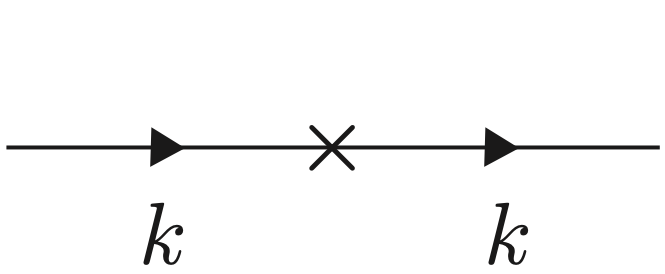
\includegraphics[width=0.2\linewidth]{pics/KG-ct.png}.
\end{aligned}
\end{equation}



\subsection{Self Energy Correction}
To second order, we consider the one-loop correction to the propagator with the diagram:
\begin{equation*}
	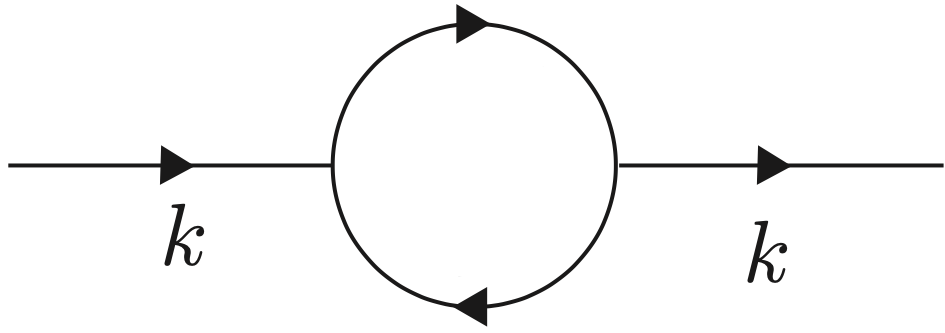
\includegraphics[width=0.3\linewidth]{pics/KG-1.png}
\end{equation*}
This correspond to 
\begin{equation}
	i\tilde{\Delta}^{(2)}(k)
	= i\tilde\Delta_0(k)\left[i\Sigma^{(2)}(k^2)\right]i\tilde\Delta_0(k), 
	\label{eq:rkg-self-energy}
\end{equation}
where the self energy term to the second order $i\Pi^{(2)}(k)$ is defined as:
\begin{equation}
	i\Sigma^{(2)}(k^2) 
	\equiv \frac{g^2}{2} \int \frac{d^dq}{(2\pi)^d} \tilde{\Delta}_0(q)\tilde{\Delta}_0(k-q) + (Ak^2-Bm^2).
\end{equation}

\begin{framedrmk}[Symmetry Factor]
The coefficient $g^2/2$ comes from the symmetry factor in the diagram. We can also check the coefficient explicitly, by considering the expansion to the second order (we denote $\delta/\delta J(x_i)$ as $\delta_i$):
\begin{equation*}
\begin{aligned}
	\delta_{1}\delta_{2}\frac{1}{2!4!}\left[\frac{ig}{3!}\int d^dy \left(\frac{\delta}{\delta J(y)}\right)^3 \right]^2
	\left[-\frac{i}{2}\int d^dy_1 d^dy_2 J(y_1)\Delta(y_1-y_2)J(y_2)\right]^4.
\end{aligned}
\end{equation*}
The expansion gives the coefficient
\begin{equation*}
	\left(\frac{ig}{6}\right)^2\times \frac{1}{2!\times 4! \times 2^4}.
\end{equation*}
Now consider the combinatorial factor, which comes from the exchange of $\phi(x_i)$ in the propagator, the exchange of $\phi(x_i)$ in the vertex, the exchange of propagator in the diagram, and the change of vertices in the diagram:
\begin{equation*}
	(2!)^4\times(3!)^2\times(4\times 3)\times2.
\end{equation*}
Those two factors produce a $-g^2/2$ coefficient.
Note that in the self energy expression (\ref{eq:rkg-self-energy}), we put a $i$ factor in front of each propagator, which absorbs the minus sign.
\end{framedrmk}

Once we obtain the self energy, the one-loop corrected propagator has the form:
\begin{equation}
\begin{aligned}
	i\tilde{\Delta}(k) 
	&= i\tilde{\Delta}_0(k) + i\tilde{\Delta}_0(k)\left[\sum_{n=1}^{\infty}i\Sigma(k^2)\right]i\tilde{\Delta}_0(k) \\
	&= \frac{i}{\tilde{\Delta}^{-1}_0(k) - \Sigma(k^2)} \\
	&= \frac{i}{k^2-m^2-\Sigma(k^2)}.
\end{aligned}
\end{equation}
Now we are going to evaluate the divergent integral in the self energy expression, using the Feynman parameters:
\begin{equation*}
\begin{aligned}
&\int \frac{d^d q}{(2 \pi)^d} \frac{1}{q^{2}-m^2} \frac{1}{(k-q)^{2}-m^2} \\
=&\int \frac{d^d q}{(2 \pi)^d} \int_{0}^{1} d x \frac{1}{\left[q^{2}-m^2+x\left((q-k)^{2}-q^{2}\right)\right]^{2}} \\
=&\int_{0}^{1} d x \int \frac{d^d q}{(2 \pi)^d} \frac{1}{\left[(q-kx)^{2}-D\right]^{2}},
\end{aligned}
\end{equation*}
where $D=m^2-k^{2} x(1-x)$. Then we can shift $q \rightarrow q+kx$ leaving an integral that only depends on $q^{2}$. In this way,
\begin{equation*}
\Sigma(k^2) = \int_0^1 I(x)dx.
\end{equation*}
To evaluate the self-energy, it suffices to obtain the integral
\begin{equation*}
I(x) = \frac{g^2}{2i}\int \frac{d^d q}{(2 \pi)^d} \frac{1}{\left[q^{2}-D\right]^{2}}.
\end{equation*}

\begin{framedrmk}[Feyman Parameters]
We use Feynman's formula to combine denominators,
\begin{equation}
\frac{1}{A_{1} \ldots A_{n}}=\int d F_{n}\left(x_{1} A_{1}+\ldots+x_{n} A_{n}\right)^{-n},
\end{equation}
where the integration measure over the Feynman parameters $x_{i}$ is
\begin{equation}
\int d F_{n}=(n-1) ! \int_{0}^{1} d x_{1} \ldots d x_{n} \delta\left(x_{1}+\ldots+x_{n}-1\right).
\end{equation}
This measure is normalized so that $\int d F_{n} =1$. 
The simplest case is
\begin{equation}
\frac{1}{A B}=\int_{0}^{1} \frac{dx}{[A+(B-A) x]^{2}}
=\int_{0}^{1} \frac{\delta(x+y-1)}{[x A+y B]^{2}} dx dy.
\end{equation}
Other useful identities are
\begin{equation}
\begin{aligned}
\frac{1}{A B^{n}} &=\int_{0}^{1} dxdy\frac{\delta(x+y-1)n y^{n-1}}{[x A+y B]^{n+1}} , \\
\frac{1}{A B C} &=\int_{0}^{1} dxdydz \frac{2\delta(x+y+z-1)}{[x A+y B+z C]^{3}} .
\end{aligned}
\end{equation}
\end{framedrmk}


By making the Wick rotation $q^0 \rightarrow i q_E^0$, the integral becomes:\footnote{
	The $d$-dimensional solid angle is
	\begin{equation}
		\Omega_d = \frac{2\pi^{d/2}}{\Gamma(\frac{d}{2})},
	\end{equation}
	where $\Gamma(x)$ is the gamma function, satisfing
	\begin{equation}
		\Gamma(1+x) = x\Gamma(x),\ 
		\Gamma(\epsilon) = \frac{1}{\epsilon}-\gamma_E + O(\epsilon).
	\end{equation}
	In particular, $\Gamma(n+1)=n!$.
}
\begin{equation*}
I(x) = \frac{g}{2}\int \frac{d^d q_E}{(2 \pi)^d} \frac{1}{\left(q_E^{2}+D\right)^{2}}
=\frac{g\Omega_d}{2(2\pi)^d} \int dq \frac{q^{d-1}}{\left(q^{2}+D\right)^{2}}.
\end{equation*}


\subsubsection*{Dimensional Regularization}
We set the dimension to $d=6-\epsilon$, and rewrite the Lagrangian as
\begin{equation}
	\mathcal L 
	= Z_{\phi}\frac{1}{2} \partial^\mu\phi\partial_\mu\phi - 
	Z_m \frac{m^2}{2}\phi^2 + Z_g\frac{g\tilde{\mu}^{\epsilon/2}}{3!}\phi^3.
\end{equation}
Note that the coupling constant should be changed to $g\rightarrow g\tilde\mu^{\epsilon/2}$ where $\mu$ is of mass dimension $[1]$ in order to get the correct dimensionality. 
We then expand the expression to zeroth order of $\epsilon$.
A useful identity is:
\begin{equation}
\int d k \frac{k^{a}}{\left(k^{2}+D\right)^{b}}
= D^{\frac{a+1}{2}-b} 
\frac{\Gamma\left(\frac{a+1}{2}\right)\Gamma\left(b-\frac{a+1}{2}\right)}{2\Gamma(b)}.
\end{equation}
Actually, we can compute the integral and series expansion in \texttt{Mathematica} all together:
\FrameTBStyle{mathematica}
\begin{lstlisting}[style=mathematicaFrameTB]
omg=(2*Pi^(d/2))/(Gamma[d/2]);
cof=g^2*\[Mu]^(6-d)/2*omg/(2*Pi)^d;
int=cof*Integrate[q^(d-1)/(q^2+D)^2,{q,0,Infinity}][[1]];
map={g^2->\[Alpha]*(4*Pi)^3,EulerGamma->Subscript[\[Gamma],E]};
ans=Series[int/.{d->6-\[Epsilon]},{\[Epsilon],0,0}];
ans/.map//Simplify
\end{lstlisting}
The result is (where $\alpha\equiv g^2/(4\pi)^3$)
\begin{equation*}
I(x)= \frac{\alpha D}{2} \left[
\ln \left(\frac{De^{\gamma_E}}{4\pi\tilde\mu^2}\right)-\left(\frac{2}{\epsilon}+1\right)
\right]+O(\epsilon).
\end{equation*}
Now insert $D=m^2-k^{2} x(1-x)$. Note that
\begin{equation*}
\int_0^1 dx D = m^2-\frac{k^2}{6}.
\end{equation*}
This simplifies the result to
\begin{equation}
	\Sigma^{(2)}(k^2) = \frac{\alpha}{2}\left(\frac{2}{\epsilon}+1\right)\left(\frac{k^2}{2}-m^2\right)
	+ \frac{\alpha}{2}\int_0^1 dx D(x)\ln\left(\frac{D(x)}{\mu^2}\right),
\end{equation}
where we have replace $\tilde\mu$ with
\begin{equation}
\mu \equiv \sqrt{\frac{4\pi}{e^{\gamma_E}}}\tilde\mu.
\end{equation}



\subsubsection*{Renormalization}
 
The counter terms also contribute to the perturbative correction,
\begin{equation*}
\begin{aligned}
	\Sigma^{(2)}\left(k^{2}\right) 
	=& \frac{\alpha}{2} \int_{0}^{1} dx D \ln\left(\frac{D}{m^{2}}\right) 
	+\left\{\frac{\alpha}{6}\left[\frac{1}{\varepsilon}+\ln\left(\frac{\mu}{m}\right)+\frac{1}{2}\right]+A\right\} k^{2} \\
	&-\left\{\alpha\left[\frac{1}{\varepsilon}+\ln\left(\frac{\mu}{m}\right)+\frac{1}{2}\right]+B\right\} m^{2}+O\left(\alpha^{2}\right) .
\end{aligned}
\end{equation*}
Consider the on-shell condition for the subtraction:
\begin{equation}
	\Sigma(m^2) = \Sigma'(m^2)=0.
\end{equation}
Set $D_0 \equiv D(x)|_{k^2=m^2}=m^2(1-x+x^2)$, the self energy has the form:
\begin{equation}
	\Sigma^{(2)}(k^2)=\frac{\alpha}{2} \int_0^1dx D(x)\ln\left(\frac{D(x)}{D_0(x)}\right) + C_k k^2+C_m m^2.
\end{equation}
The condition $\Pi(m^2) =0$ requires
\begin{equation*}
	\Sigma^{(2)}(k^2)=\frac{\alpha}{2} \int_0^1dx D(x)\ln\left(\frac{D(x)}{D_0(x)}\right) + C_k (k^2-m^2).
\end{equation*}
The condition $\Pi'(m^2)=0$ requires
\begin{equation*}
\begin{aligned}
	\left.\frac{d\Sigma^{(2)}(k^2)}{dk^2}\right|_{k^2=m^2}
	&=\frac{\alpha}{2} \int_0^1dx \left.\left[
	\frac{D(x)}{dk^2}\ln\left(\frac{D(x)}{D_0(x)}\right)+D_0(x)
	\right]\right|_{q^2=m^2} + C_k  \\
	&= \frac{\alpha}{2}\int_0^1dx (x^2-x) + C_k \\
	&= C_k-\frac{\alpha}{12} = 0.
\end{aligned}
\end{equation*}
In this way, we obtained the renormalized self-energy:
\begin{equation}
	\Sigma^{(2)}(k^2)=\frac{\alpha}{2} \int_0^1dx D(x)\ln\left(\frac{D(x)}{D_0(x)}\right) + \frac{\alpha}{12}(k^2-m^2).
\end{equation}

On the other hand, we chan choose the $\overline{\mathrm{MS}}$ subtraction scheme, i.e.,
\begin{equation}
	A = -\frac{\alpha}{6\epsilon},\ 
	B = -\frac{\alpha}{\epsilon}.
\end{equation}
The self energy under $\overline{\mathrm{MS}}$ scheme will depend on the the mass scale $\mu$ we choose:
\begin{equation}
	\Sigma^{(2)}\left(k^{2}\right) 
	= \frac{\alpha}{2} \int_{0}^{1} dx D \ln\left(\frac{D}{m^{2}}\right) 
	+\alpha\left[\ln\left(\frac{\mu}{m}\right)+\frac{1}{2}\right]\left(\frac{k^2}{6}-m^2\right).
\end{equation}


\subsection{Vertex Correction}
Now consider the simplest one-loop correction to the vertex function from the diagram:
\begin{equation*}
	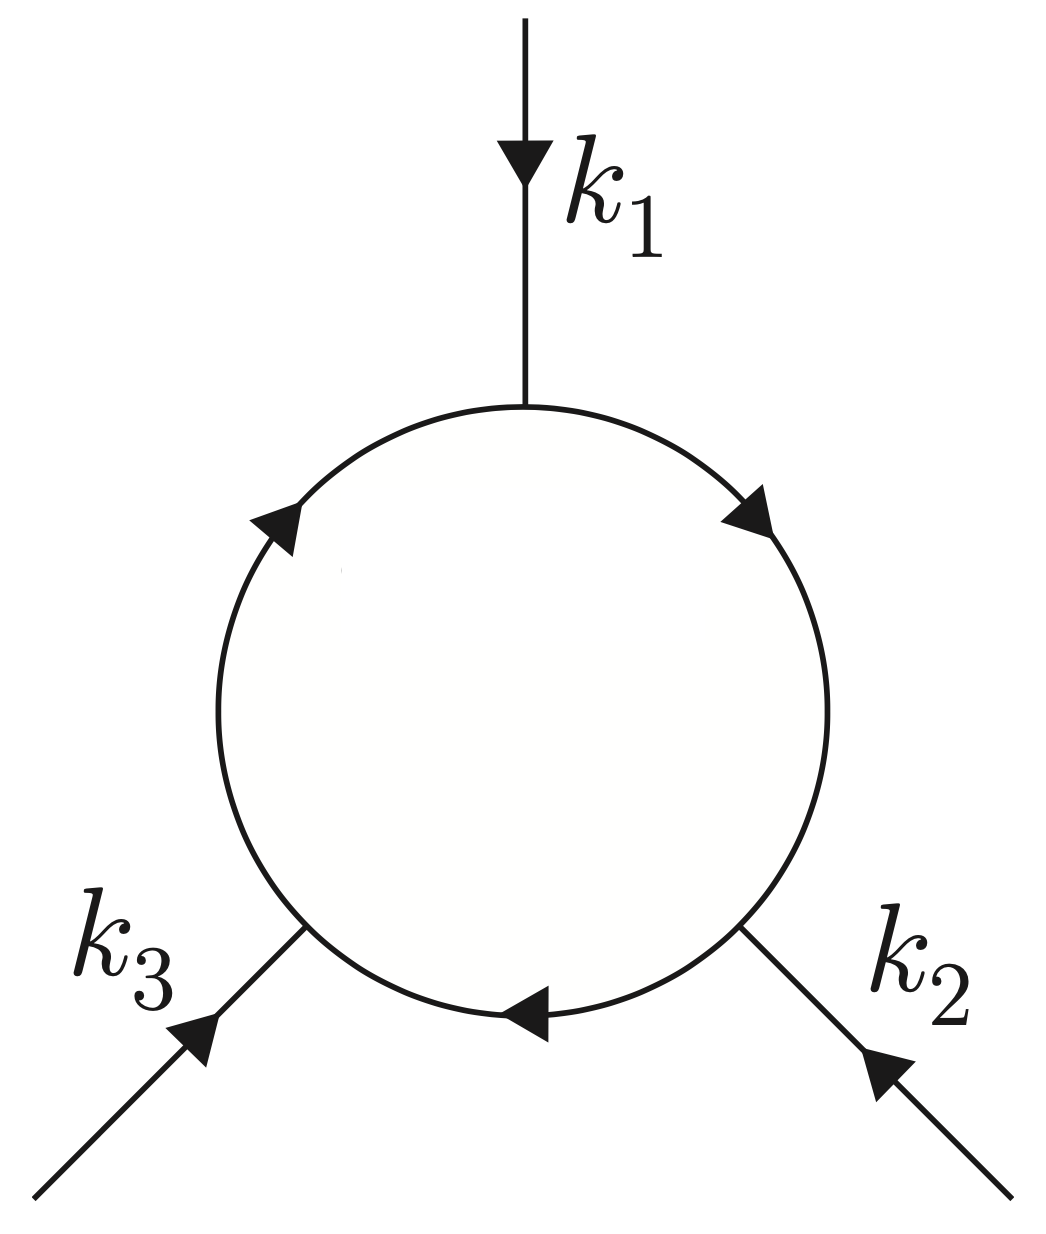
\includegraphics[width=0.23\linewidth]{pics/KG-2.png}
\end{equation*}
The vertex function corresponding to such correction, together with the counter term, can be expressed as:
\begin{equation}
	i V_3^{(3)}(k_{1}, k_{2}, k_{3})
	= (ig)^3i^3 \int \frac{d^{a} q}{(2 \pi)^{d}} \tilde{\Delta}(q-k_{1}) \tilde{\Delta}(q+k_{2}) \tilde{\Delta}(q) + i Cg,
\end{equation}
Using the Feynman parameter, the integrant is
\begin{equation*}
\tilde{\Delta}(q-k_{1}) \tilde{\Delta}(q+k_{2}) \tilde{\Delta}(q) 
= \int d F_3\frac{1}{(q^2-D)^3}
\end{equation*}
where we have shift the value of $q$, and $D$ can be evaluate by the following code:
\begin{lstlisting}[style=mathematicaFrameTB]
A1=(l-k1)^2-m^2;
A2=(l+k2)^2-m^2;
A3=(l)^2-m^2;
{c,b,a}=CoefficientList[x1*A1+x2*A2+(1-x1-x2)*A3,{l}];
-c+b^2/(4*a)//Expand
\end{lstlisting}
The result is
\begin{equation*}
D = m^2-k_1^2 x_1 (1- x_1)-k_2^2 x_2 (1- x_2)-2 k_1 k_2 x_1 x_2.
\end{equation*}
The same procedure gives:
\begin{equation}
	V_3^{(3)}/g = \int dF_3 I(x_1,x_2,x_3) + C,
\end{equation}
where
\begin{equation*}
I(x_1,x_2,x_3) = \frac{g^2 \Omega_d}{(2\pi)^d} \int dq \frac{q^{d-1}}{(q^2+D)^3}.
\end{equation*}
The same regularization procedure in \texttt{Mathematica}:
\begin{lstlisting}[style=mathematicaFrameTB]
omg=(2*Pi^(d/2))/(Gamma[d/2]);
cof=g^2*\[Mu]^(6-d)*omg/(2*Pi)^d;
int=cof*Integrate[q^(d-1)/(q^2+D)^3,{q,0,Infinity}][[1]];
map={g^2->\[Alpha]*(4*Pi)^3,EulerGamma->Subscript[\[Gamma],E]};
ans=Series[int/.{d->6-\[Epsilon]},{\[Epsilon], 0, 0}];
ans/.map//Simplify
\end{lstlisting}
The result is
\begin{equation}
\begin{aligned}
	V_3^{(3)}/g 
	&= \frac{\alpha}{\epsilon}
	+ \frac{\alpha}{2}\int dF_3 \ln\left(\frac{4\pi\tilde{\mu}^2e^{-\gamma_E}}{D}\right) 
	+ C + O(\epsilon) \\
	&= \frac{\alpha}{\epsilon}
	+ \alpha\ln\left(\frac{\mu}{m}\right)
	- \frac{\alpha}{2}\int dF_3 \ln\left(\frac{D}{m}\right)
	+C.
\end{aligned}
\end{equation}
The on-shell subtraction requires 
\begin{equation}
V_3(0,0,0) = g,
\end{equation}
which gives
\begin{equation}
	C = -\frac{\alpha}{\epsilon}-\alpha \ln\left(\frac{\mu}{m}\right).
\end{equation}
So the vertex function to the third order is
\begin{equation}
	V_3(k_1,k_2,k_3) = g\left\{1-\frac{\alpha}{2} \int dF_3 \ln\left[\frac{D(x_1,x_2,x_3)}{m}\right] \right\}.
\end{equation}
The $\overline{\mathrm{MS}}$ scheme, on the other hand, sets
\begin{equation}
	C = -\frac{\alpha}{\epsilon}.
\end{equation}



\subsection{Renormalization Group}
We fist summarize the normalization factor obtained on the one-loop level (with $\overline{\mathrm{MS}}$ subtraction scheme):
\begin{equation}
\begin{aligned}
	Z_{\phi} &= 1-\frac{\alpha}{6\epsilon} + O(\alpha^2), \\
	Z_{m} &= 1-\frac{\alpha}{\epsilon}+ O(\alpha^2), \\
	Z_{g} &= 1-\frac{\alpha}{\epsilon}+ O(\alpha^2).
\end{aligned}
\end{equation}
For the renormalized Lagrangian in ($6-\epsilon$)-dimension
\begin{equation}
	\mathcal L 
	= Z_{\phi}\frac{1}{2} \partial^\mu\phi\partial_\mu\phi - 
	Z_m \frac{m^2}{2}\phi^2 + Z_g\frac{g\tilde{\mu}^{\epsilon/2}}{3!}\phi^3,
\end{equation}
the factors relate the original field and bare coefficients
\begin{equation}
	\phi_0 = Z_\phi^{1/2}\phi,\ 
	m_0 = Z_m^{1/2} Z_\phi^{-1/2}m,\ 
	g_0 = Z_g Z_{\phi}^{-3/2} \tilde{\mu}^{\epsilon/2}g.
\end{equation}
The renormalization group requires that the bare parameter is independent of the mass scale $\mu$ we choose, that is:
\begin{equation}
	\frac{d\phi_0}{d \ln \mu} 
	= \frac{dm_0}{d \ln \mu}
	= \frac{dg_0}{d \ln \mu}
	= 0.
\end{equation}


\subsubsection*{Beta Function}
Star with $g_0$, it is more convenient to use 
\begin{equation}
\alpha_0 
\equiv \frac{g_0^2}{4\pi} 
= Z_g^2 Z_{\phi}^{-3}\tilde{\mu}^{\epsilon}\alpha.
\end{equation}
Take logarithm on both side:
\begin{equation}
\ln \alpha_0 = \ln(Z_g^2 Z_{\phi}^{-3}) 
+ \ln \alpha + \epsilon\ln{\tilde\mu}.
\end{equation}
The RG equation is
\begin{equation}
\frac{d \ln \alpha_0}{d \ln \mu} = 
\frac{d \ln(Z_g^2 Z_{\phi}^{-3}) }{d \alpha}\frac{d \alpha}{d\ln \mu} +
\frac{1}{\alpha}\frac{d \alpha}{d \ln \mu} + \epsilon
=0.
\end{equation}
To the first order of $\alpha$:
\begin{equation}
\begin{aligned}
	\frac{d \ln(Z_g^2 Z_{\phi}^{-3}) }{d \alpha}
	=\frac{d}{d\alpha}\left(-\frac{2\alpha}{\epsilon}+\frac{\alpha}{2\epsilon}\right) 
	= -\frac{3}{2\epsilon},
\end{aligned}
\end{equation}
which leads to
\begin{equation}
	\frac{d\alpha}{d\ln \mu}\left(1-\frac{3\alpha}{2\epsilon}+O(\alpha^2)\right)+\epsilon\alpha = 0.
\end{equation}
The beta function is defined as
\begin{equation}
	\beta(\alpha) = \frac{d\alpha}{d\ln \mu} = \beta_1 \alpha + \beta_2 \alpha^2 + O(\alpha^3).
\end{equation}
Insert such definition into the original expression, and keep track of the order of $\alpha$, we get
\begin{equation}
	(\beta_1+\epsilon)\alpha + \left(\beta_2-\frac{3\beta_1}{2\epsilon}\right)\alpha^2 + O(\alpha^3) = 0.
\end{equation}
The beta function is
\begin{equation}
	\beta(\alpha) = -\epsilon \alpha -\frac{3}{2}\alpha^2 + O(\alpha^3).
\end{equation}



\subsubsection*{Anomalous Dimension}
Consider the RG equation with bare mass:
\begin{equation}
\begin{aligned}
\frac{d\ln m_0}{d\ln \mu} 
&= \frac{1}{2}\frac{d(\ln Z_m - \ln Z_\phi)}{d\alpha}\frac{d\alpha}{d\ln\mu}
	+\frac{1}{m}\frac{d m}{d\ln \mu} \\
&= \frac{5\alpha}{12}+\frac{1}{m}\frac{d m}{d\ln \mu} + O(\alpha^2) = 0.
\end{aligned}
\end{equation}
We get the anomalous dimension of the mass:
\begin{equation}
\gamma_m(\alpha) \equiv \frac{1}{m}\frac{d m}{d\ln \mu} 
= -\frac{5\alpha}{12}+O(\alpha^2).
\end{equation}
Also, for the bare field
\begin{equation}
\frac{d\ln\phi_0}{d\ln\mu} = \frac{1}{2} \frac{d\ln Z_{\phi}}{d\ln\mu} 
+ \frac{d\ln\phi}{d\ln\mu} = 0.
\end{equation}
We can define the anomalous dimension of the field as
\begin{equation}
\gamma_{\phi} \equiv \frac{1}{2}\frac{d \ln Z_\phi}{d\ln\mu}
= \frac{1}{2}\frac{d \ln Z_\phi}{d\alpha}\frac{d\alpha}{d\ln\mu}
= \frac{\alpha}{12} +O(\alpha^2).
\end{equation}



\subsubsection*{Callan-Symanzik Equation}
Consider the bare propagator:
\begin{equation}
\tilde{\Delta}_0(k) = Z_\phi \tilde{\Delta}(k)
\end{equation}
The RG condition for the bare propagator gives:
\begin{equation*}
\frac{d\ln\tilde{\Delta}_0(k)}{d \ln\mu}
=\frac{d\ln Z_\phi}{d\ln\mu}+\frac{1}{\tilde{\Delta}(k)}\left(
	\frac{\partial}{\partial\ln\mu} +
	\frac{d\alpha}{d\ln\mu}\frac{\partial}{\partial\alpha} +
	\frac{dm}{d\ln\mu}\frac{\partial}{\partial m}
\right)\tilde{\Delta}(k)=0.
\end{equation*}
The Callan-Symanzik equation is
\begin{equation}
	\left(
	2\gamma_\phi+
	\frac{\partial}{\partial\ln\mu} +
	\beta(\alpha)\frac{\partial}{\partial\alpha} +
	\gamma_m(\alpha)m\frac{\partial}{\partial m}
\right)\tilde{\Delta}(k)=0.
\end{equation}

\section{$\phi^4$ Theory on 4D Space-time}
In this section, we consider the real Klein-Gordon field with $\phi^4$ interaction in ($4-\epsilon$)-dimension space-time:
\begin{equation}
	\mathcal{L}
	= Z_{\phi}\frac{1}{2} \partial^\mu\phi\partial_\mu\phi - 
	Z_m \frac{m^2}{2}\phi^2 - Z_g\frac{g \tilde{\mu}^\epsilon}{4!}\phi^4.
\end{equation}
Note that the field $\phi$ has mass dimension $[\frac{d-2}{2}]=[1]$, so the original coupling constant $g$ is dimensionless.

As the $\phi^3$ theory, we can rewrite the Lagrangian as:
\begin{equation}
	\mathcal L = \mathcal L_0 + \mathcal L_{\mathrm{int}} + \mathcal L_{\mathrm{ct}}.
\end{equation}
In the following we investigate the loop correction to the mass and the coupling constant.


\subsection{One-loop Correction}
\subsubsection*{Self-energy}
Following the same procedure, the one-loop self-energy correction is
\begin{equation}
	i\Sigma(k^2) = -\frac{g\tilde{\mu}^\epsilon}{2}\int \frac{d^d q}{(2\pi)^d} \frac{1}{q^2-m^2} + i(Ak^2-Bm^2).
\end{equation}
The first term comes from the diagram
\begin{equation*}
	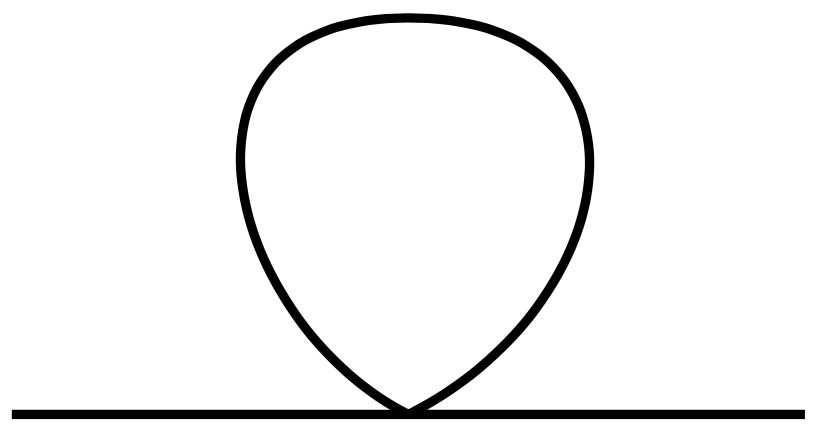
\includegraphics[width=0.2\linewidth]{pics/KG-3.png}
\end{equation*}
and the second term comes from the counter terms. 
After the Wick rotation, 
\begin{equation}
	\Sigma(k^2) = -\frac{g\tilde{\mu}^\epsilon}{2}\frac{\Omega_d}{(2\pi)^d} \int \frac{q^{d-1} dq}{q^2+m^2} + (Ak^2-Bm^2).
\end{equation}
The dimensional regulation is carried out using the following code:
\begin{lstlisting}[style=mathematicaFrameTB]
omg=(2*Pi^(d/2))/(Gamma[d/2]);
cof=g*\[Mu]^(4-d)/2*omg/(2*Pi)^d;
int=cof*Integrate[q^(d-1)/(q^2+m^2),{q,0,Infinity}][[1]];
map={EulerGamma->Subscript[\[Gamma],E]};
ans=Series[int/.{d->4-\[Epsilon]},{\[Epsilon],0,0}];
ans/.map//Simplify
\end{lstlisting}
The result is
\begin{equation}
	\Sigma(k^2) = \frac{g m^2}{32\pi^2} \left[\frac{2}{\epsilon}+1+\log \left(\frac{4 \pi \tilde{\mu}^2 e^{-\gamma_E}}{m^2}\right)\right]+(Ak^2-Bm^2)+O(\epsilon).
\end{equation}
Using the $\overline{\mathrm{MS}}$ renormalization scheme, we set
\begin{equation}
	A = 0,\ B = \frac{g}{16\pi^2\epsilon}.
\end{equation}
The result is
\begin{equation}
	\Sigma(k^2) = \frac{g m^2}{16\pi^2} \log \left(\frac{\mu}{m}\right)
	+\frac{g m^2}{32\pi^2}+O(\epsilon).
\end{equation}

\subsubsection*{Vertex Correction}
Now consider the vertex correction.
To the lowest order the diagram is
\begin{equation*}
	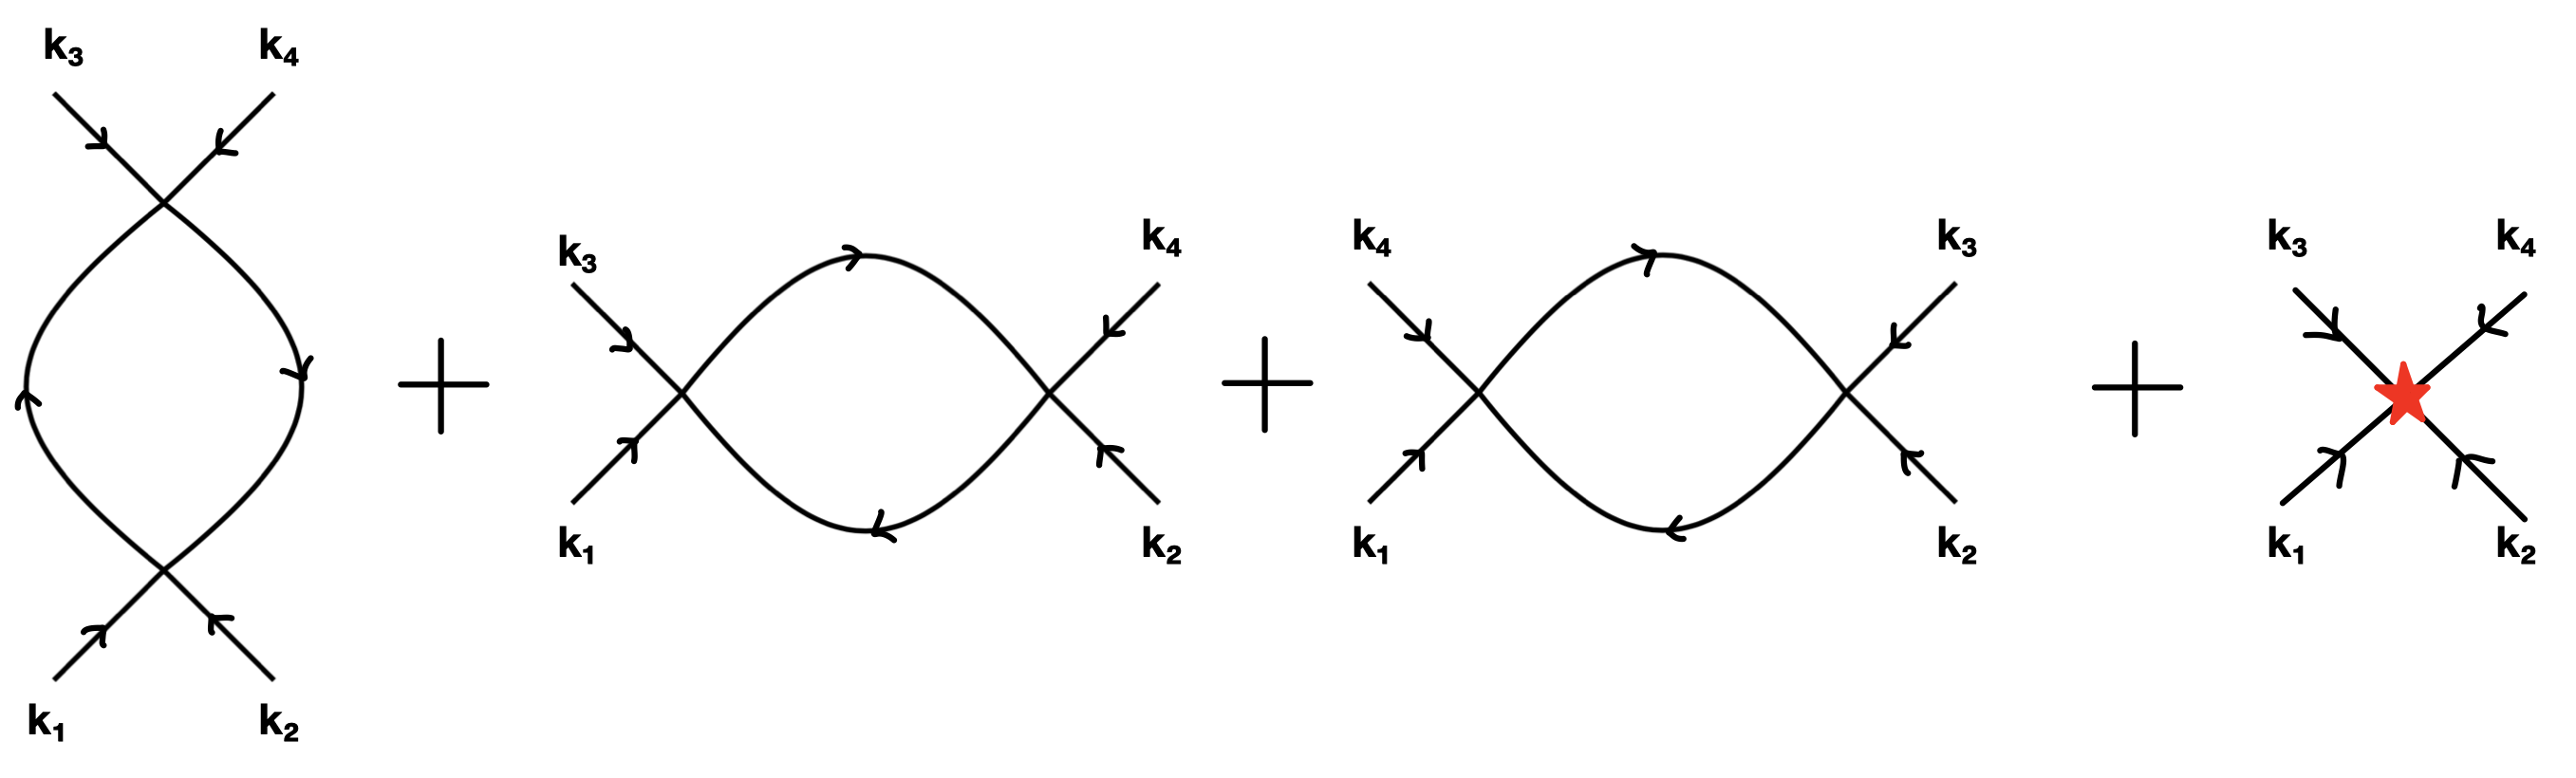
\includegraphics[width=0.2\linewidth]{pics/KG-4.png}
\end{equation*}
Together with the counter term, the vertex function is
\begin{equation}
	iV_4^{(2)}(k_1,k_2,k_3,k_4) = \frac{g^2}{2} \left[iF(s)+iF(t)+iF(u)\right] -iCg,
\end{equation}
where
\begin{equation}
	s = (k_1+k_2)^2,\ 
	t = (k_1+k_3)^2,\ 
	u = (k_1+k_4)^2,
\end{equation}
and
\begin{eqnarray}
	iF(k^2) 
	&=& \tilde{\mu}^{\epsilon}\int \frac{d^d q}{(2\pi)^d} \tilde{\Delta}_0(q)\tilde{\Delta}_0(q+k) \\
	&=& \frac{i\tilde{\mu}^{\epsilon}\Omega_d}{(2\pi)^d} \int_0^1 dx \int \frac{q^{d-1}dq}{\left[q^2+m^2+x(1-x)k^2\right]^2}.
\end{eqnarray}
Then we carry out the calculation (set $D(k^2,x)=m^2+x(1-x)k^2$)
\begin{lstlisting}[style=mathematicaFrameTB]
omg=(2*Pi^(d/2))/(Gamma[d/2]);
cof=g^2*\[Mu]^(4-d)/2*omg/(2*Pi)^d;
int=cof*Integrate[q^(d-1)/(q^2+D)^2,{q,0,Infinity}][[1]];
map={EulerGamma->Subscript[\[Gamma],E]};
ans=Series[int/.{d->4-\[Epsilon]},{\[Epsilon],0,0}];
ans/.map//Simplify
\end{lstlisting}
The result is:
\begin{equation}
\begin{aligned}
	F(s) &= \frac{1}{8\pi^2\epsilon} + \frac{1}{16\pi^2}\int_0^1 dx \ln \left(\frac{4\pi \tilde{\mu}^2 e^{-\gamma_E}}{D}\right) \\
	&= \frac{1}{8\pi^2\epsilon} +\frac{1}{8\pi^2}\ln \left(\frac{\mu}{m}\right) - \frac{1}{16\pi^2}\int_0^1 dx \ln\left(\frac{D(s,x)}{m^2}\right).
\end{aligned}
\end{equation}
The $\overline{\mathrm{MS}}$ scheme absorbs the $\frac{1}{8\pi^2\epsilon}$ term, i.e.,
\begin{equation}
	C = \frac{3g}{16\pi^2}.
\end{equation}
The result is:
\begin{equation}
	V_4(k_1,k_2,k_3,k_4) = -g+\frac{g^2}{32\pi^2}\int_0^1 dx \ln\left(\frac{\mu^6}{D(s,x)D(t,x)D(u,x)}\right).
\end{equation}
To summarize, the normalization is:
\begin{eqnarray}
	Z_{\phi} &=& 1, \\
	Z_{m} &=& 1+\frac{g}{16\pi^2 \epsilon}, \\
	Z_{g} &=& 1+\frac{3g}{16\pi^2 \epsilon}.
\end{eqnarray}


\subsection{Renormalization Group}
Now consider the RG equation for the one-loop correction. 
The bare parameters are:
\begin{equation}
	g_0 = Z_g g\tilde{\mu}^{\epsilon},\ 
	m_0 = Z_m^{1/2} m,
\end{equation}
The RG conditions are:
\begin{eqnarray}
	\frac{d g_0}{d\ln \mu}
	&=& \left(\frac{3}{16\pi^2 \epsilon} + \frac{1}{g}\right)\frac{dg}{d\ln \mu} + \epsilon = 0, \\
	\frac{d m_0}{d\ln \mu}
	&=& \frac{1}{32\pi^2 \epsilon}\frac{dg}{d\ln \mu} + \frac{1}{m}\frac{dm}{d \ln \mu} = 0.
\end{eqnarray}
Consider the series expansion of beta function:
\begin{equation}
	\beta(g) = \frac{dg}{d\ln \mu} = \beta_1 g + \beta_2 g^2 +O(g^3).
\end{equation}
The beta function is
\begin{equation}
	\beta(g) = -\epsilon g + \frac{3g^2}{16\pi^2} + O(g^3).
\end{equation}
The anomalous dimension of mass is
\begin{equation}
	\gamma_m = \frac{1}{m}\frac{dm}{d \ln \mu} = \frac{g}{32\pi^2}+O(g^2)
\end{equation}



